% !TEX TS-program = xelatex
% !TEX encoding = UTF-8 Unicode

\providecommand{\home}{../..}
\documentclass[\home/main.tex]{subfiles}

\begin{document}

\chapter{Learning to fold through cloth instrumentation}\label{ch:instrumentation}

In simulation environments, fully estimating the state of cloth is trivial because any point can be queried for information (\cref{ch:simulation}).
For example, bringing a cloth into a known configuration by grasping the corners can be done by querying the location of the corner points in simulation and planning a grasping trajectory.
In the real world, finding corner points is more difficult due to sensor noise and self-occlusions. \cref{ch:lit} concluded that existing folding research estimates the cloth state only in simulation or by using cameras and visual trackers in the real world. This chapter steps away from the vast focus on vision-based solutions and explores an alternative approach by embedding tactile sensing within a cloth and training a classifier to enable a smart cloth to communicate its own state. We show how this smart textile can be used for learning to fold a cloth on a low-cost, dual robotic arm.

First, we give a summary of our motivation for researching alternatives to vision-based cloth state estimation in \cref{sec:instrumentation_lit}. We refer to \cref{ch:lit} in this book for a full review on the existing literature on cloth state estimation. Next, we introduce the robotic platform we utilize in our experiments in \cref{sec:instrumentation_robotic_setup}. \cref{sec:instrumentation_smart_cloth} introduces our smart cloth technology and \cref{sec:instrumentation_results} discusses the real-world folding results we achieved with it.
We provide a discussion on our future perspectives on grippers and cloth instrumentation in \cref{sec:instrumentation_discussion}.
Finally, \cref{sec:instrumentation_conclusion} summarizes the main findings of our work on instrumentation.

\section{Vision-based state estimation of cloth} \label{sec:instrumentation_lit}

% DISTILLED PREV RELATED WORK
When calculating the required trajectories for deformable object manipulation, the deformations need to be taken into account \autocite{Foresti2004}. One approach to incorporate deformations is in simulation where the state is fully accessible.
% SIM and sim2real problem
For example, \textcite{Matas2018} use deep \gls{RL} to train a neural network to learn to manipulate a towel. The reward signal consists of the simulated cloth state and the policies learned in simulation are transferred to the real platform using domain randomization. In their approach, the agent learns from the pixel input only, while tactile sensing coud lead to a more informational representation of the cloth. Another approach is to learn a forward dynamics model of the cloth in simulation \autocite{Tanaka2018}. The learned dynamics model can then be used to bring cloth into the desired configuration. In our own work (\cref{ch:simulation}), we calculated the distance between corner points that need to be close together in order to achieve a fold (\cref{eq:sim_cost_function}). However, transferring results in simulation to the real world have proven to be challenging due to the difficulty in generating high-fidelity, simulated rollouts.

% State estimation op echt cloth
Sim2Real issues render state estimation of cloth in the physical setup a viable alternative.
% State estimation op echt cloth - for engienered pipelines
State estimation methods rely heavily on detecting points of interest like the corners of clothes. \textcite{Maitin2010}, for example, regrasp a cloth until a corner point is found. However, this process is the largest bottleneck in their system, taking up to 24 minutes to fold a shirt.
% State estimation op echt cloth - for RL pipelines
State estimation is also a requirement for \gls{RL} approaches to cloth folding: a reward function is required to signal task success \autocite{Tsurumine2019, Matas2018}.
\textcite{Balaguer2011} apply visual marks on a towel in order to track the state. The markings allow calculating the distance between points on the towel from the training sample and the example demonstrations so that it can be used as a reward for the agent. Their method requires prior information about the shape of the object in order to reconstruct the missing market points.
However, relying solely on visual inputs and marker clues does not scale well. Another approach to find a reward function was explored in \autocite{Abbeel2004, Finn2016}, where inverse reinforcement learning (IRL) was used to learn a reward function from expert demonstrations. Because IRL learns a reward function and a policy separately, it requires RL to be run in an inner loop, making it computationally expensive to train. Learning the reward function offline decouples reward learning and policy learning and makes training on a real robot feasible.

% Conclusie: vision OK maar we willen touch :D
% our motivation for researching alternative approaches to vision-based state estimation of cloth, 
To conclude, a typical approach for the robotic folding of textile relies on the use of vision in order to detect grasping points and to perform texture segmentation and pose estimation \autocite{Maitin2010, Doumanoglou2016, Bersch2011}, as well as to estimate the state \autocite{Matas2018} and---in the case of reinforcement learning (RL)-based approaches---the reward function \autocite{Tsurumine2019}. However, while vision is instrumental for recognizing and localizing objects, touch and force measurements become important once contact occurs and the object is explored using the end-effector \autocite{Billard2019}. Recent work \autocite{Tian2019} has illustrated this idea by applying a touch-based control method for a ball repositioning task, rolling a dice and the deflection of a stick. In line with other authors \autocite{Tian2019, Lee2019}, we believe the use of tactile input and its fusion with other sensory information is crucial to learn complex robot manipulation tasks in an efficient way.

%===============================================================================

\section{Dual-arm robotic setup} \label{sec:instrumentation_robotic_setup}

% \subsection{Dual-arm robotic setup}

Cloth manipulation is inherently bimanual because a second grasp is required for most tasks to bring cloth into desired configurations. There exist bimanual robotic platforms like Baxter\textregistered\ and PR2\textregistered. However, the spirit behind our research for instrumentation is one of democratization of hardware. A PR2 robot, for example, can cost \SI{400000}[\$]{}. Sensors similar to the one we are proposing to construct, require advanced and financially expensive tools like photonic sintering systems \autocite{You2016sensor}.
We aim to use off-the-shelf components and a DIY approach to instrumentation and robotics research. For this reason, we constructed the BCN3D Moveo robot arms\footnote{\url{https://github.com/BCN3D/BCN3D-Moveo}}. The Moveo arm is an open-source initiative to enable the robotics community to build a low-cost robotic arm. The arm has five degrees of freedom. It can be fabricated by rapid prototyping techniques and off-the-shelf components. We show a picture of the constructed Moveo arm in \cref{fig:moveo_arm}.

\begin{figure}[htpb]
    \centering
    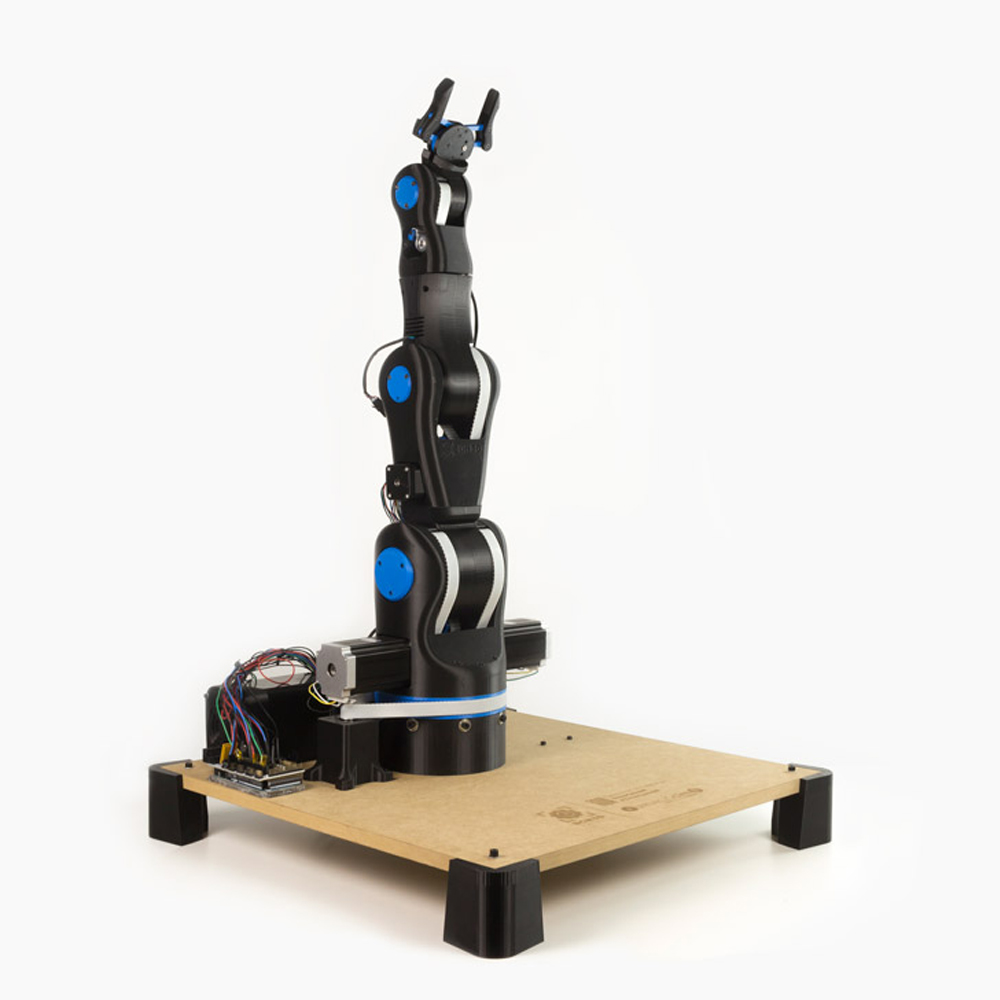
\includegraphics[width=0.9\textwidth, keepaspectratio]{figures/moveo_arm}
    \caption{Picture of the constructed Moveo arm. TODOOOOOOOOOOOOOOOOOOOOOOOOO}
    \label{fig:moveo_arm}
\end{figure}

The task we propose is folding a rectangular patch of smart textile. We only consider the manipulation task of folding the cloth and assume the textile is already grasped by attaching the cloth to the two-fingered gripper by means of a hook-and-loop fastener. We place the arms opposable as visible in the setup in \cref{fig:setup_overview}.

\begin{figure}[htpb]
    \centering
    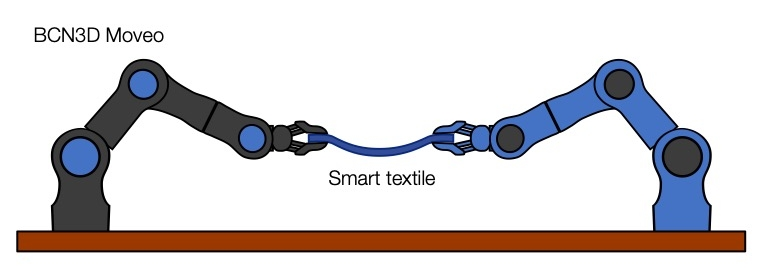
\includegraphics[width=0.9\textwidth, keepaspectratio]{figures/folding_overview_smaller.jpg}
    \caption{Schematic overview of the setup: dual robot arms hold a smart textile piece and have to learn to fold it from scratch using sensory feedback of the textile and proprioceptive input of the robotic~arms. }
    \label{fig:setup_overview}
\end{figure}

%===============================================================================

\section{Smart cloth} \label{sec:instrumentation_smart_cloth}

To detect the folded state of the cloth, we propose creating a smart cloth with integrated tactile sensing. We can then record a dataset of cloth states associated with sensor values to train a classifier that is able to recognize whether the cloth is folded. We first discuss the hardware options and our tactile sensing implementation, followed by our methodology and results to train a smart cloth.


% However, this requires the detection of the state of the cloth---a~non-trivial task given the high amount of cloth configurations. Hand-engineered heuristics to estimate the cloth state have been researched \autocite{Doumanoglou2016} but are highly complex to reproduce and are prone to error. Visual cues such as colored surfaces or fiducial markers \autocite{Bersch2011, Tsurumine2019} can be attached to highly deformable materials but require the many occlusions caused by the self-collision of the cloth to be~handled.

\subsection{Tactile sensing technologies}
While tactile sensing always seems to be lagging behind compared to vision \autocite{Siciliano2008}, the field has been growing in recent years \autocite{Chi2018}. This growth can be attributed to novel fabrication methods \autocite{Zou2017} and a renewed interest in multimodal sensing for robotics \autocite{digit2020}.
A complete overview of tactile sensing technologies can be found in \autocite{Siciliano2008} with updates about recent developments in \autocite{Zou2017,Chi2018}. This section gives a short overview and discusses tradeoffs concerning various tactile sensing solutions.

The transduction mechanisms for external forces differ widely in the following properties: sensitivity, resolution, dynamic range, cost, ease of production and reliability. Common transduction mechanisms are capacitive, piezoresistive, piezoelectric and optical \autocite{Chi2018}.
Capacitive pressure sensing arrays form capacitors by separating a grid of electrodes by a dielectric material. A deformation in the dielectric material then induces a change in capacitance. Capacitive sensors are characterized by having high sensitivity and resolution but requires dealing with noise due to stray capacitances.
Piezoresistive sensors operate on the principle of variable resistors: the change in resistance of a material acts as a proxy for force sensing. These sensors have a simple working principle and are low-cost to fabricate. For example, the strain gauge is a popular piezoresistive sensing technology available in many DIY electronics shops.
Piezoelectric materials generate charges when being subjected to forces. However, the induced charges dissipate quickly, making it hard to use piezoelectric sensors to detect static contact. This is necessary when it is required to, for example, detect whether the cloth is still being grasped.
Optical sensors analyze changes of internal light or track optical markers inscribed on a membrane. For tactile sensing with robot fingers, a growing class of visuotactile sensors measures the deformation of a gel or a membrane. Examples are GelSight \autocite{Yuan2017}, Soft-bubble \autocite{Naveen2020fast} and Digit \autocite{digit2020}. However, we scope our requirements to tactile sensing to be embedded inside clothing. Hence, the used technology should exert minimal influence on the deformable properties of the textile.

For robotics in general, capacitive and piezoresistive are popular choices due to the mentioned advantages. Our application requires the sensing technology to be low-cost, accessible to fabricate and contain a high degree of sensitivity to detect folds. Piezoresistive sensors are simple and low-cost to produce, and have a high spatial resolution. The dynamic range can be configured with the fixed reference resistor in front of the variable resistor material. The low reproducibility of different piezoresistive sensors can be mitigated by using machine learning methods trained on different, uncalibrated batches of sensors. This makes piezoresistive sensing technology for our case more suitable compared to capacitive sensing, which requires relatively more complex measurements circuits to read out the capacitances and deal with noise and cross-talk.

\subsection{Cloth sensing using piezoresistive rubber}

The general principle behind the piezoresistive sensor is to construct a matrix of variable resistors. The voltage over the variable resistors is related to the pressure and can be calculated via the voltage divider principle shown in \cref{fig:instrumentation_voltage_divider}. The voltage $V$ over a variable resistor $R$ becomes:
\begin{equation}
    V=\frac{R_{A}}{R_{A}+R} \cdot \mathrm{~V}_{in}
\end{equation}
with $R_A$ being the fixed resistor that can be optimized to maximize the range of $V$.
\begin{figure}[htpb]
    \centering
    \subfile{figures/fig-voltage-divider.tex}
    \caption{The voltage divider measures the voltage $V$ over the variable resistor $R$ and uses the fixed resistor $R_A$ as reference.}
    \label{fig:instrumentation_voltage_divider}
\end{figure}

Our implementation uses a piezoresistive rubber, commercially available as Velostat\textsuperscript{\textregistered}. Velostat is a polymer injected with a carbonaceous powder called carbon black that provides electrical properties similar to graphite \autocite{Dzedzickis2020}. By compressing Velostat, the carbon particles get pushed together, increasing the conductivity of the material.

The electrodes can be organized into a grid with a single or double layer.
The first option to form a single layer of electrodes is visible in \cref{fig:instrumentation_sensor_pad}. This design allows placing the electrical components on a flexible PCB with a Velostat layer on top. We show one of our implementations in \cref{fig:instrumentation_flex_pcb}. The individual pressing points, called taxels, are measured by applying a reference voltage on the row electrode and iterating through the column points while measuring the input voltage on their input pins. The data is processed locally on the sensor by using an ATtiny1634 microprocessor. While this design integrates naturally for robotic fingertips, we found the electrodes in the copper wire to be fragile, the production cost is higher than two-layered copper threads and less scalable to integrate into the textile due to miniaturization on the flexible PCB.

\begin{figure}[htpb]
    \centering
    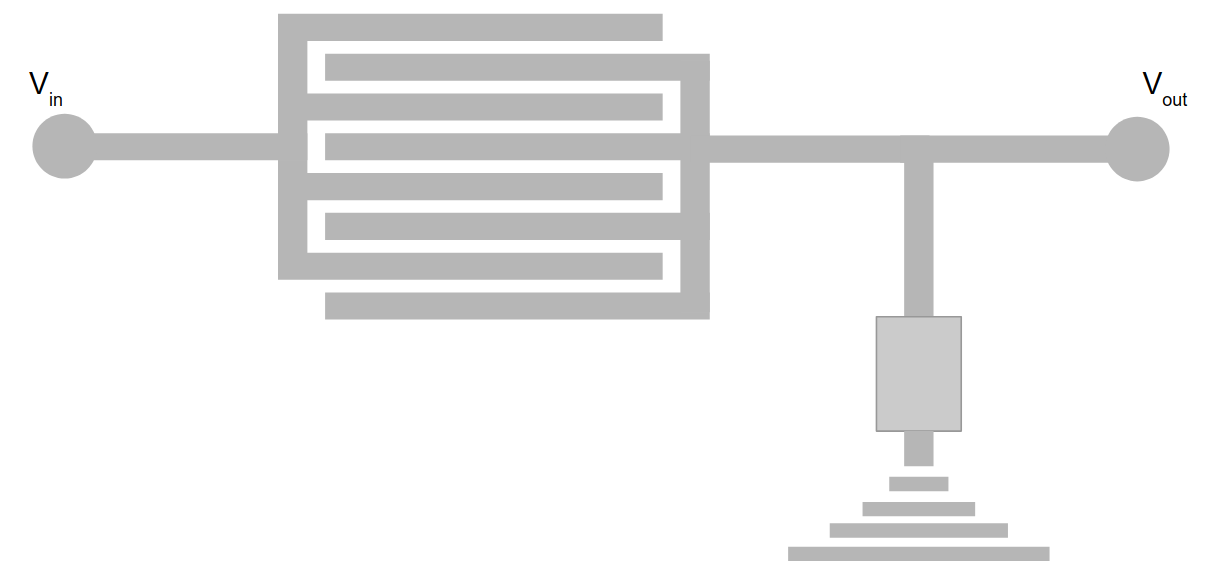
\includegraphics[width=\textwidth]{figures/sensor-pad-principle}
    \caption{Schematic presentation of electrodes of a piezoresistive sensor organized in a single-layered pad.}
    \label{fig:instrumentation_sensor_pad}
\end{figure}

\begin{figure}[htpb]
    \centering
    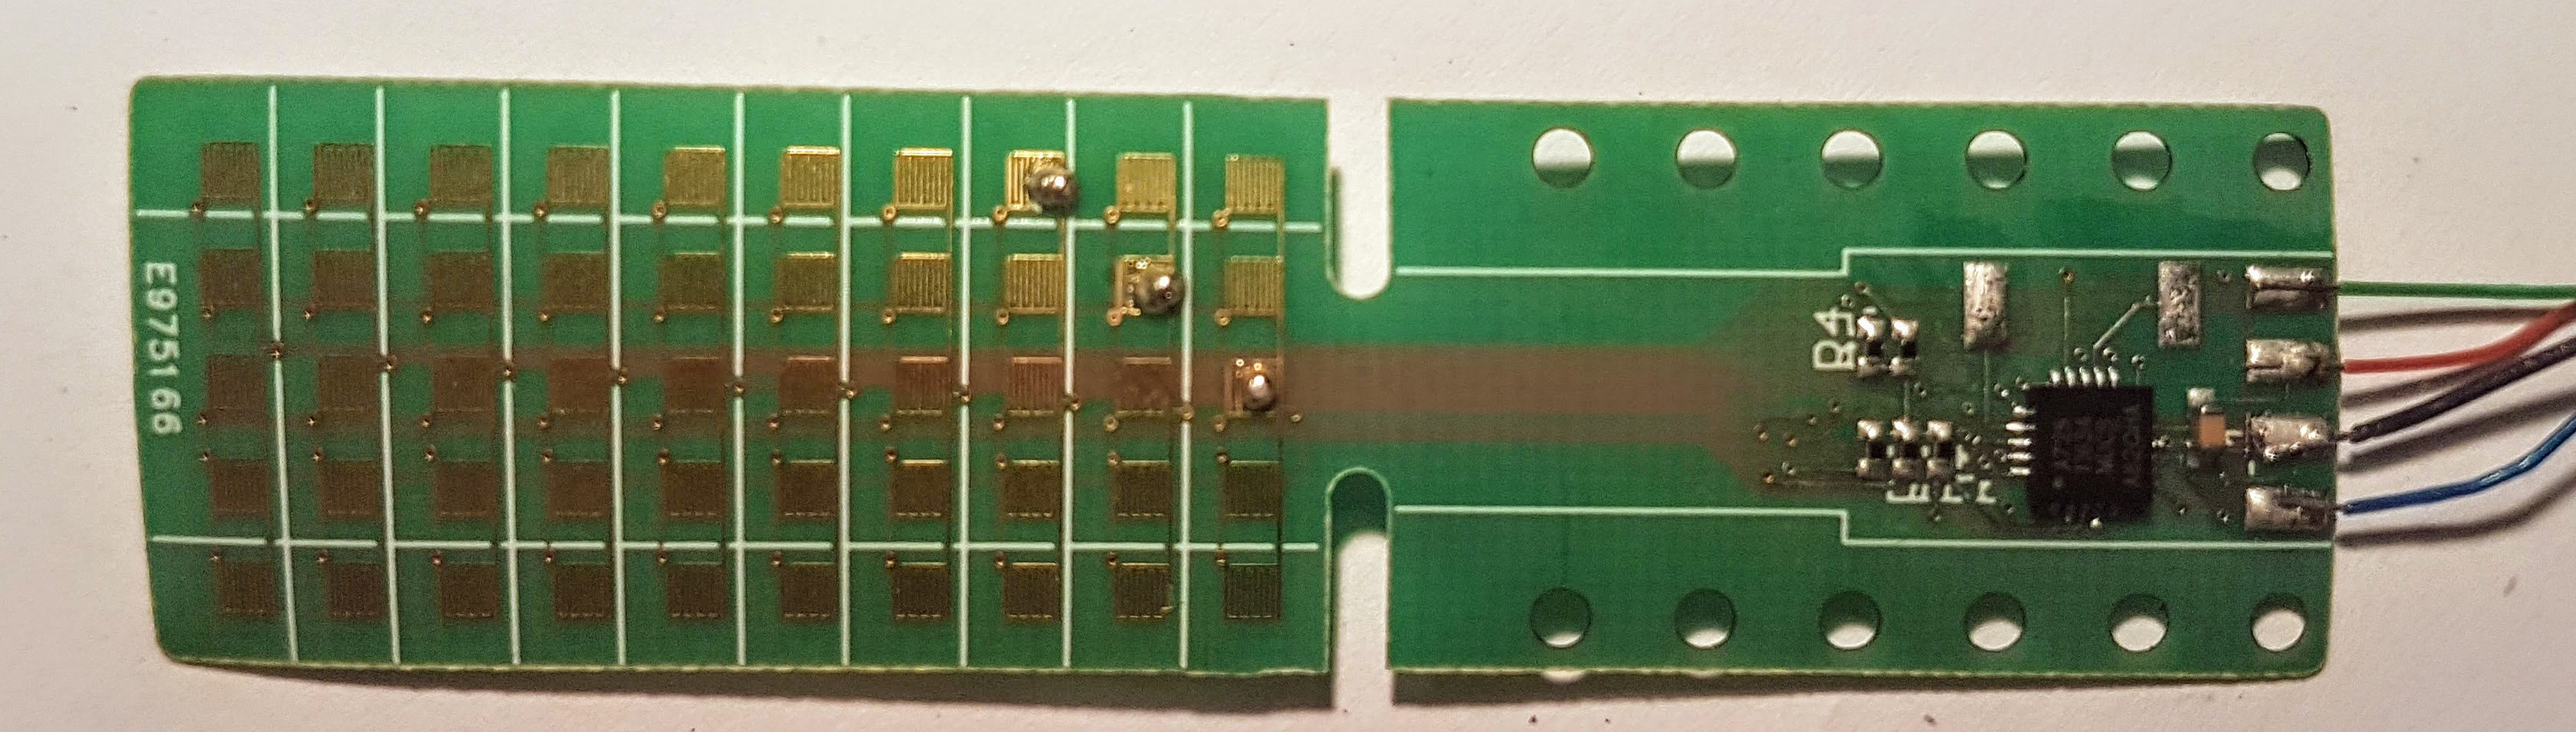
\includegraphics[width=\textwidth]{figures/flex_pcb}
    \caption{Our production of a piezoresistive sensor with electrodes in a single layer printed on a \qty{0.2}{\milli\meter} thin, flexible PCB.}
    \label{fig:instrumentation_flex_pcb}
\end{figure}

Instead of organizing the electrodes in a single layer, we create a grid using a layer with horizontal electrodes and a second layer with vertical electrodes. The electrodes are made of copper strips that are insulated with a polyimide film. We sandwich the Velostat between these two conductive layers. The layers in the smart textile can be seen in Figure~\ref{fig:textile_scheme}. This results in a matrix of $12$ by $7$ tactile cells. The signal conditioning for measuring the pressure applied over a tactile cell is based on the above-mentioned voltage divider principle. More specifically, the~voltage is measured between the tactile cell, which acts as a variable resistor, and a fixed resistor $R_A$ of \qty{5.6}{\kilo\ohm}. A standard microcontroller, a Arduino MKR WiFi 1010, measures and processes the voltage. A LiPo battery powers the circuit and the wireless WiFi module of the Arduino allows communicating with the cloth remotely.

\begin{figure}[htpb]
    \centering
    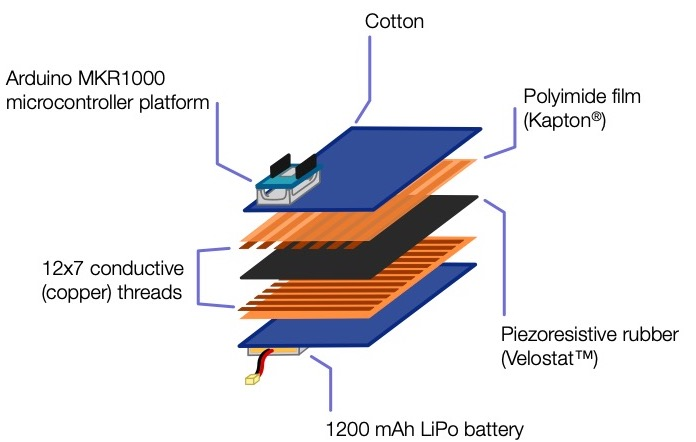
\includegraphics[width=0.85\textwidth, keepaspectratio]{figures/textile_overview.jpg}
    \caption{Exploded-view drawing of the textile with integrated tactile sensing. Conductive threads organized in a 12 by 7 grid are applied on piezoresistive rubber, creating a variable resistor. The~resulting voltage acts as a proxy for local forces applied on the cloth. }
    \label{fig:textile_scheme}
\end{figure}

Finally, the stacked layers of electronics is embedded in a cotton sleeve to form a smart cloth. The resulting textile can be seen in \cref{fig:textile_real}. The electronics slightly influence the cotton's deformability, although we have not quantified the change in deformability. However, the primary deformable characteristic of the cotton is not changed, making it suitable for folding experiments. The main component making the cotton stiffer is the Velostat sheet of \qty{0.1}{\milli\meter} thickness and weights roughly \qty{15}{\gram}. The wires have a lesser impact because they run to the terminal endpoints of the copper electrodes, as can be seen in the zoom-in photo in \cref{fig:textile_real_electronics}.

\begin{figure}[htpb]
    \centering
    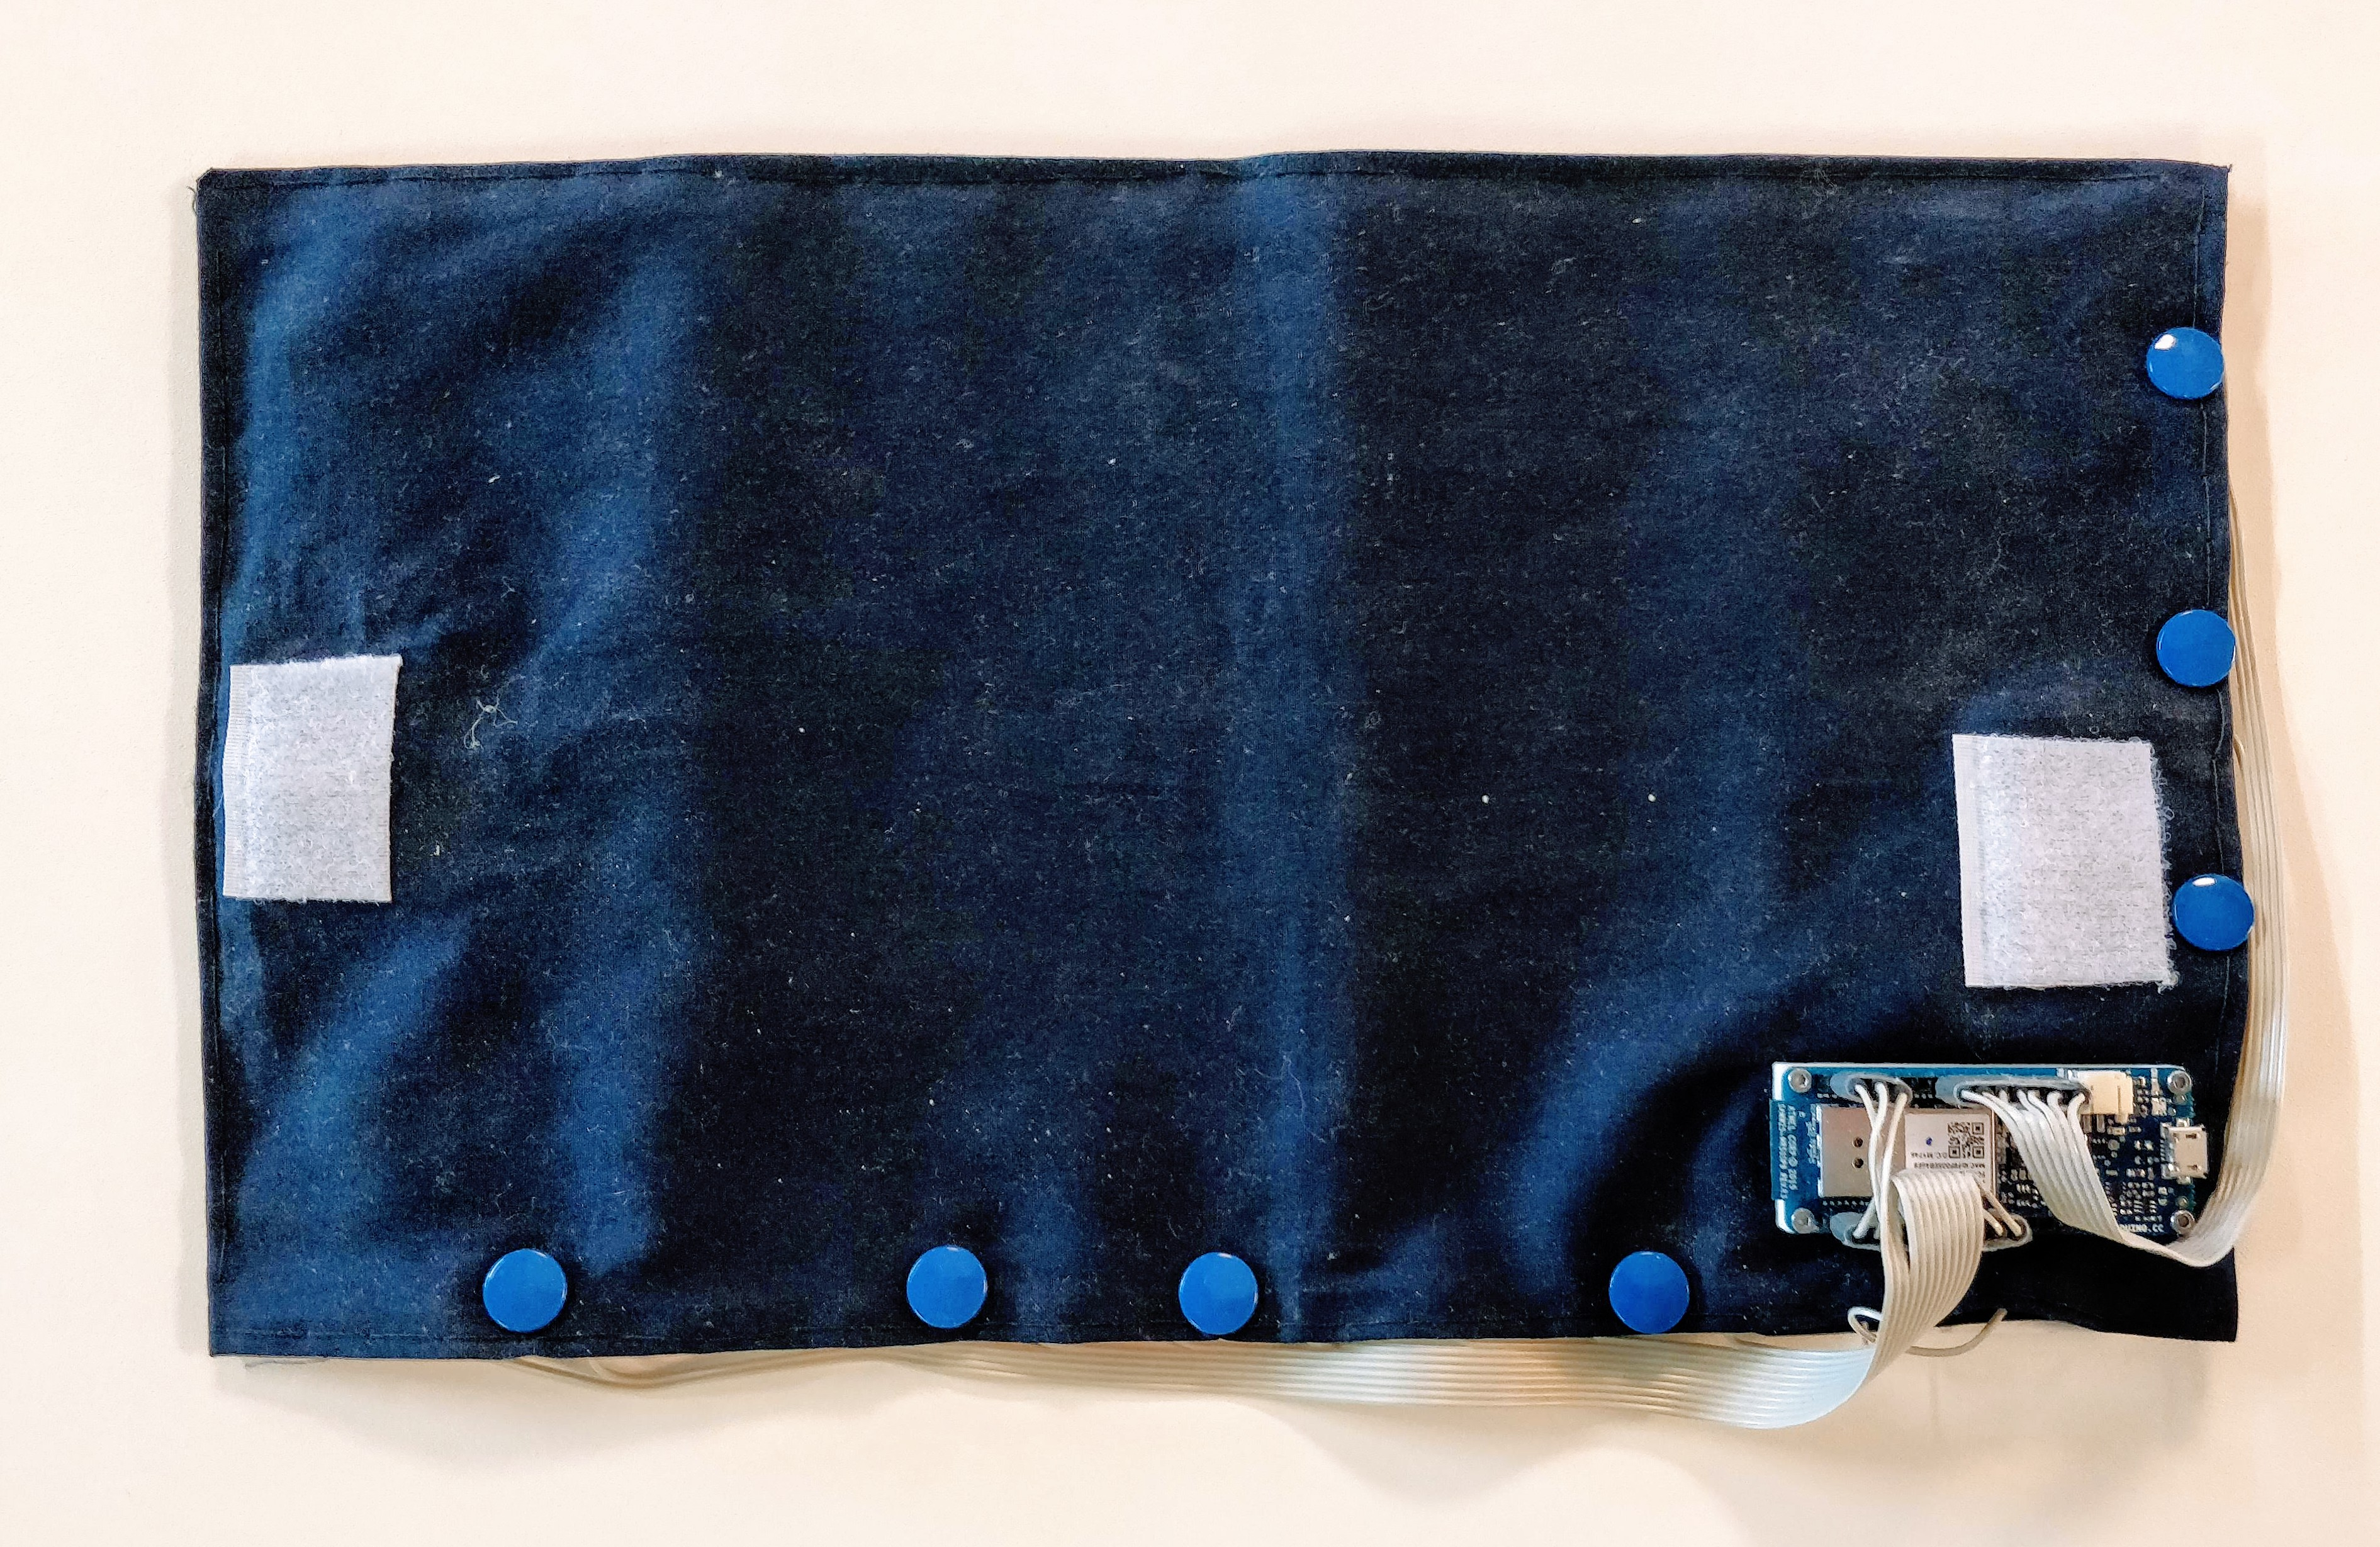
\includegraphics[width=0.90\textwidth, keepaspectratio]{figures/textile.jpg}
    \caption{Our resulting implementation of a smart textile which is able to detect and translate local forces to a state configuration (for example, folded or unfolded). The smart textile is made using accessible off-the-shelf materials and tools.}
    \label{fig:textile_real}
\end{figure}

\begin{figure}[htpb]
    \centering
    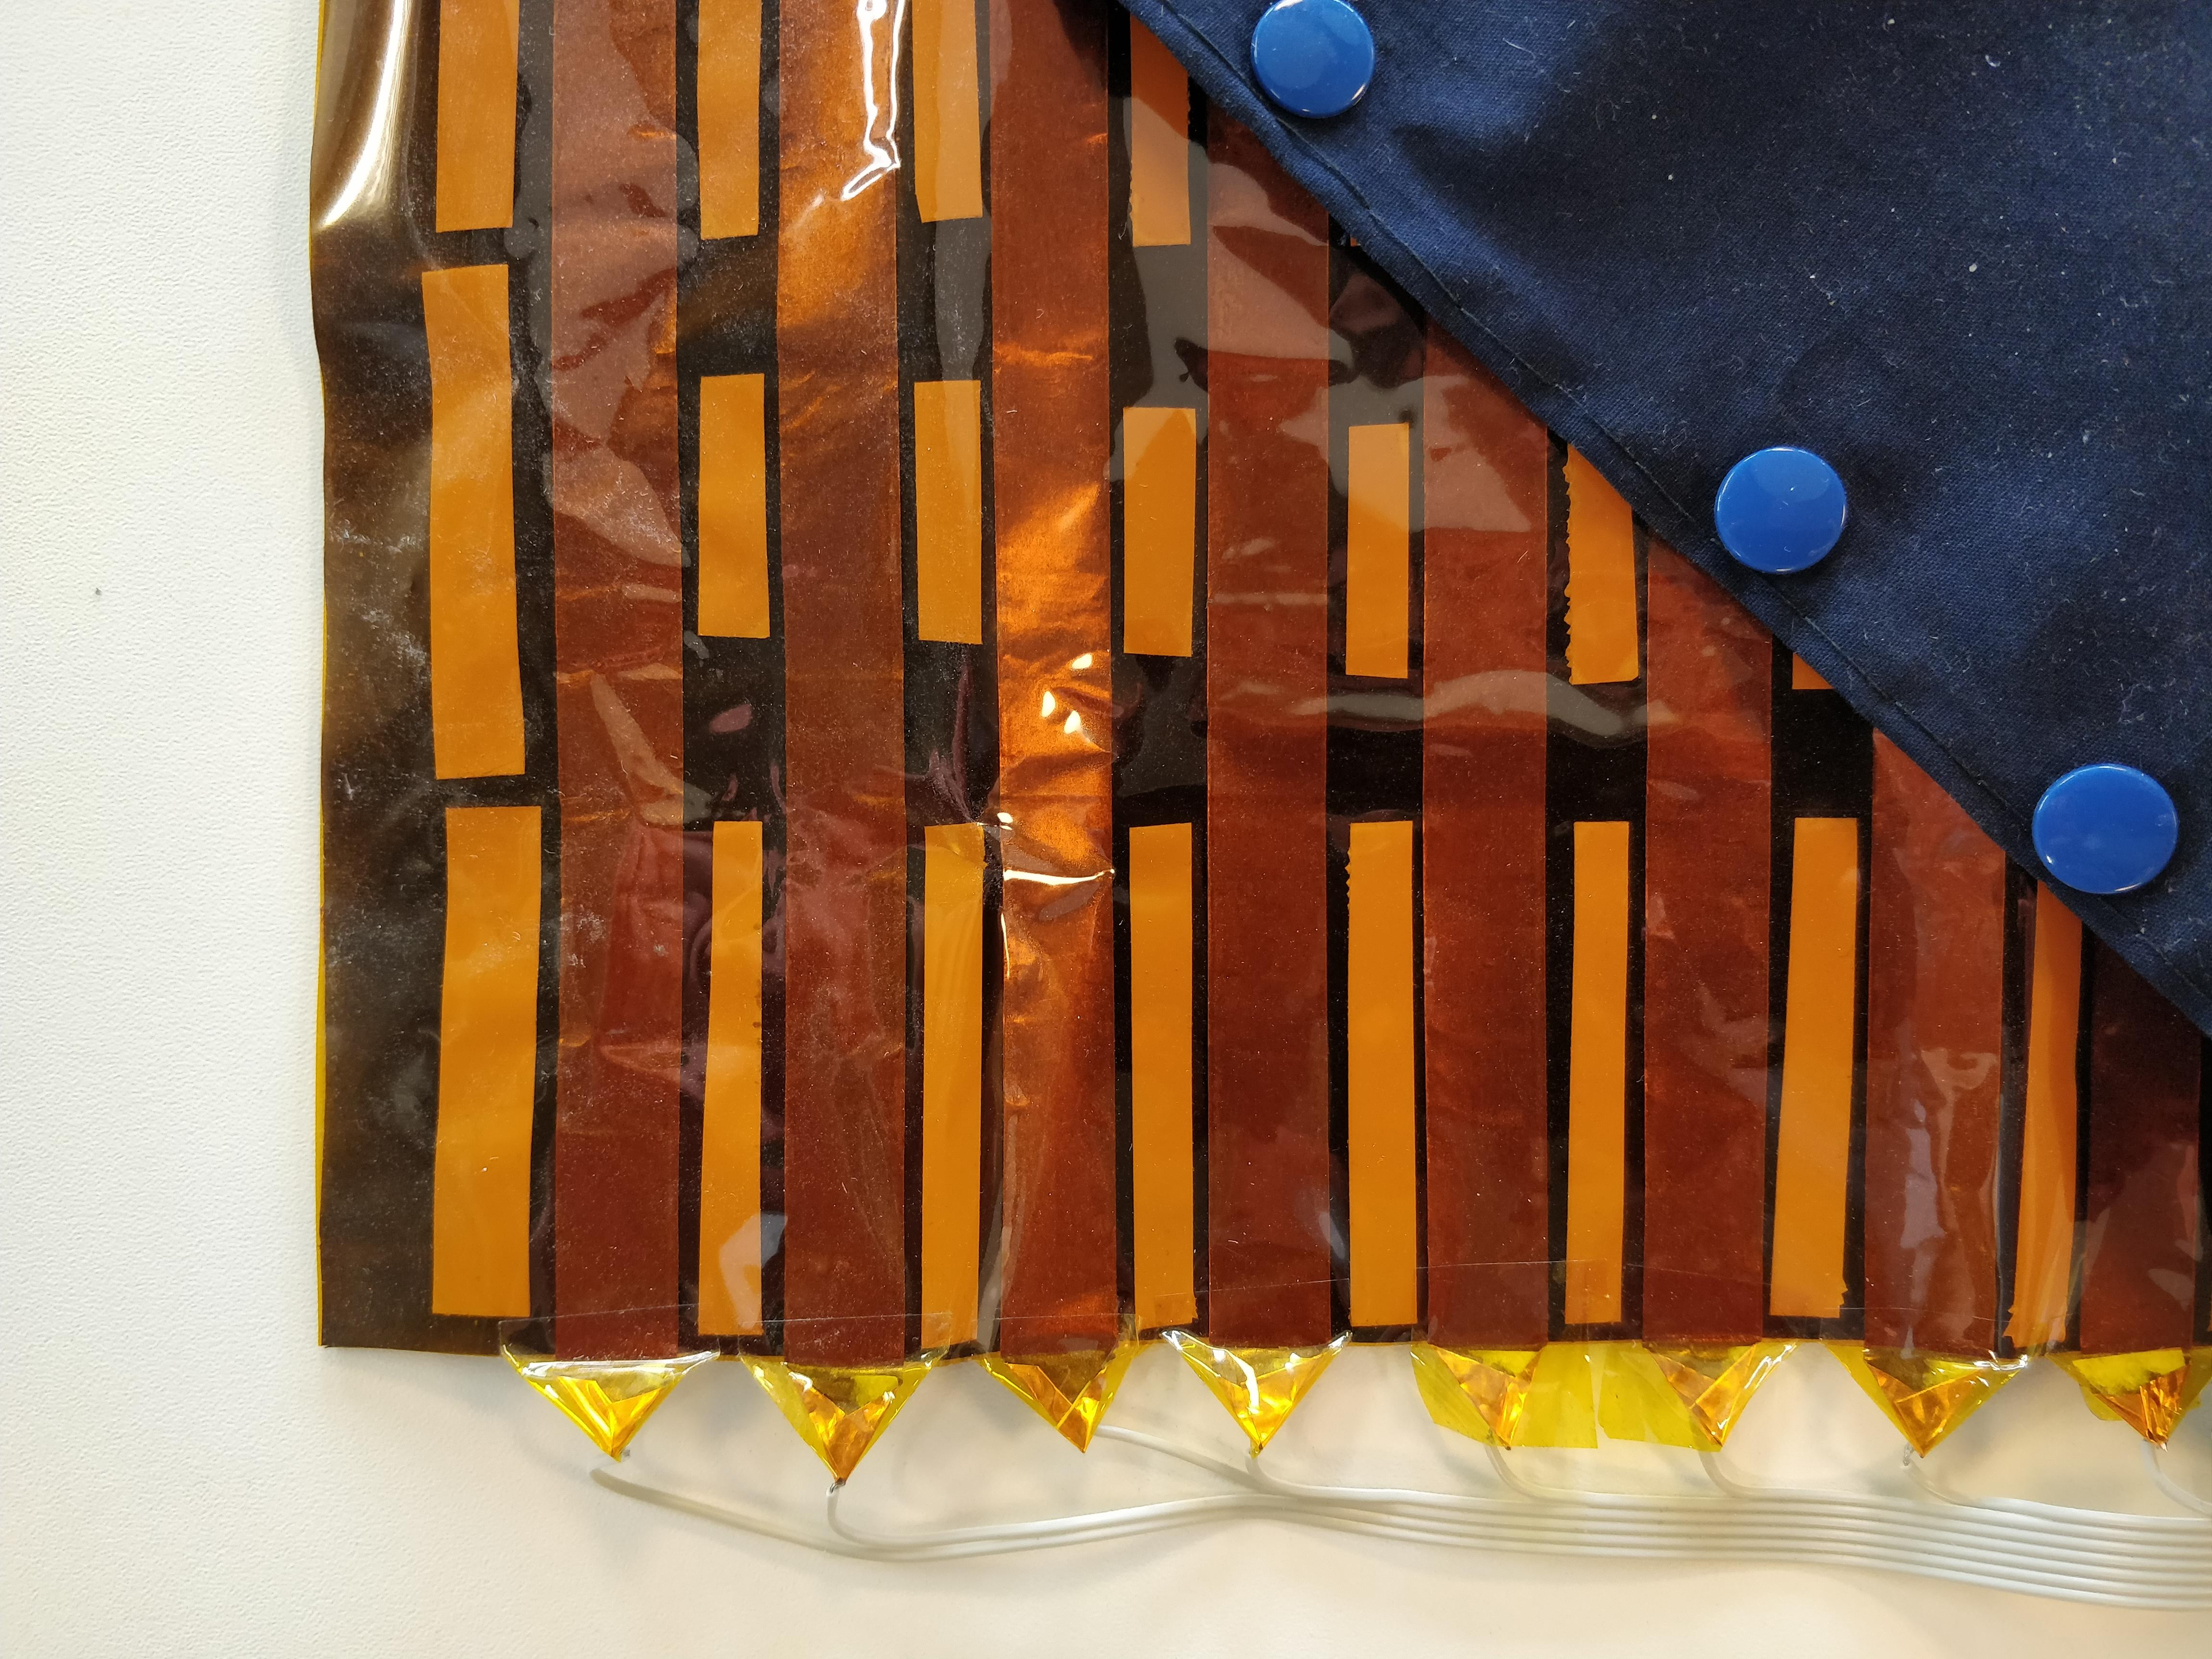
\includegraphics[width=0.90\textwidth, keepaspectratio]{figures/img-electronics-smart-textile.jpg}
    \caption{Zoom-in photo on the electronics embedded in our  smart textile.}
    \label{fig:textile_real_electronics}
\end{figure}



\subsection{Learning a smart cloth}
We aim to use the integrated tactile sensors to make the textile able to sense and react to its surrounding environment, making it an active smart textile \autocite{Stoppa2014}. To make the cloth smart, we train a linear classifier to predict the garment state: folded or unfolded. Therefore, we first collected data from the 12 by 7 tactile cells by bringing the cloth into multiple configurations while hand-labelling the associated state. We define the folded state of the cloth with some slack because of the way in which the robots are positioned in order to avoid a collision; this is illustrated in \cref{fig:folded_real}. The collected data were split into a training set of \qty{1418}{} samples and a test set of 511 samples. In \cref{fig:sensor_data}, the average voltage and standard deviation of the tactile cells for both garment states are shown. One can observe that there is a clear voltage peak in the centre column, implying that the tactile cells in the centre of the textile experience higher pressure due to the folded~state.

\begin{figure}[htpb]
    \centering
    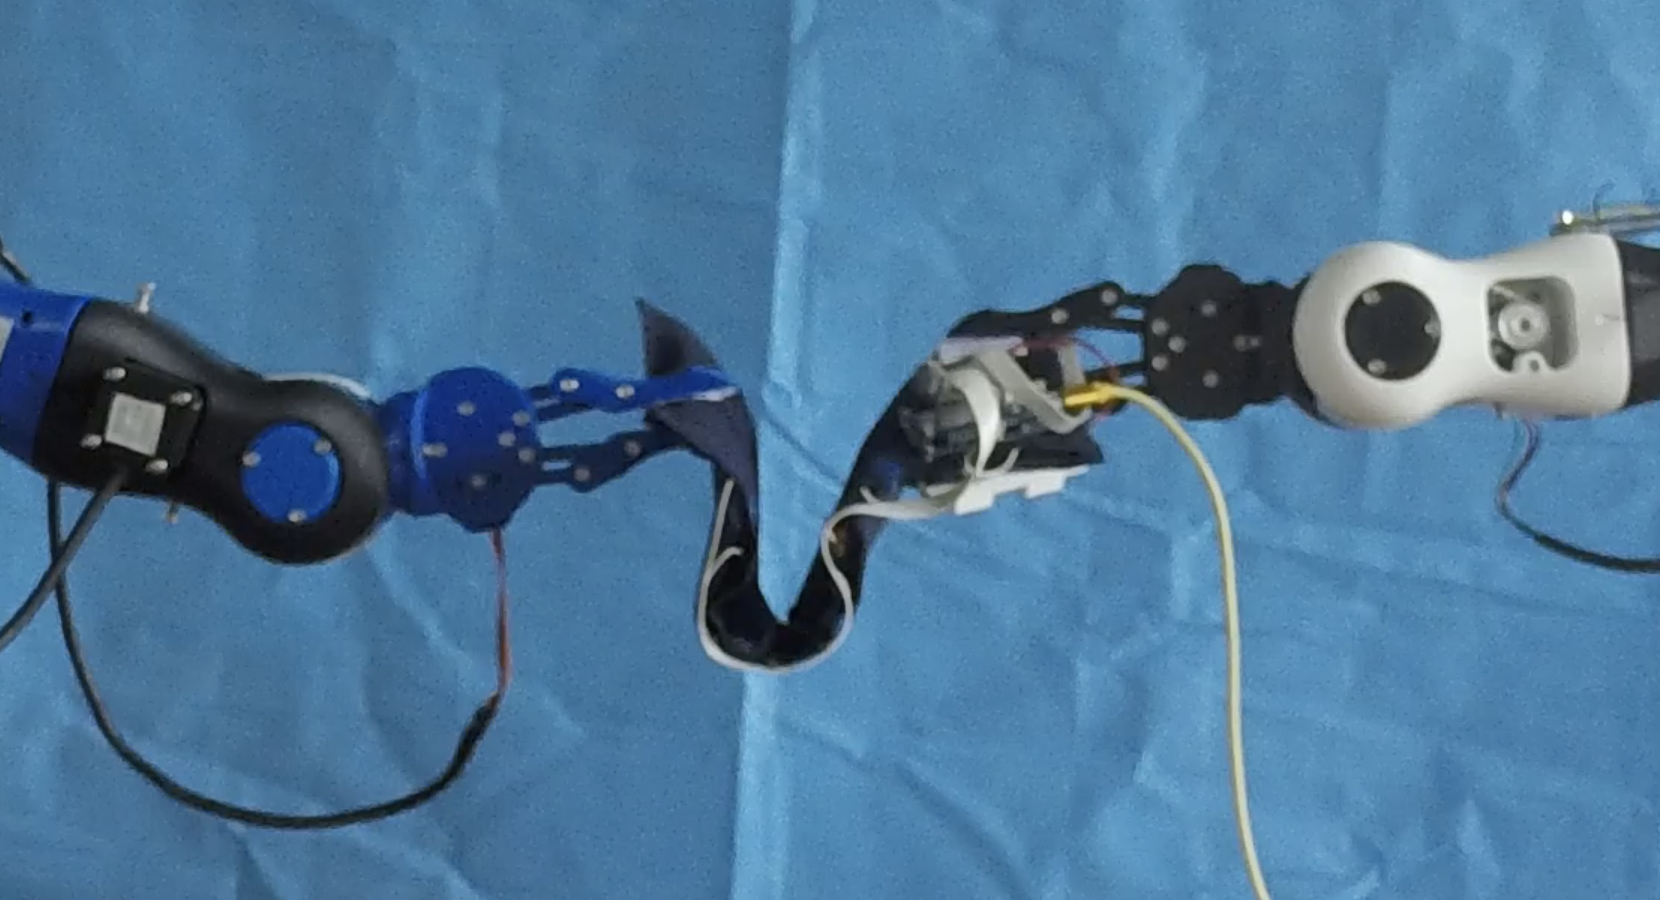
\includegraphics[width=0.90\textwidth, keepaspectratio]{figures/folded_real.png}
    \caption{Example of the folding task on the real platform. The robotic arms are positioned in such a way that they cannot collide, making it physically impossible to fold the cloth fully. Thus, we do not require a fully folded state of the textile from the agent.}
    \label{fig:folded_real}
\end{figure}

\begin{figure}[htpb]
    \centering
    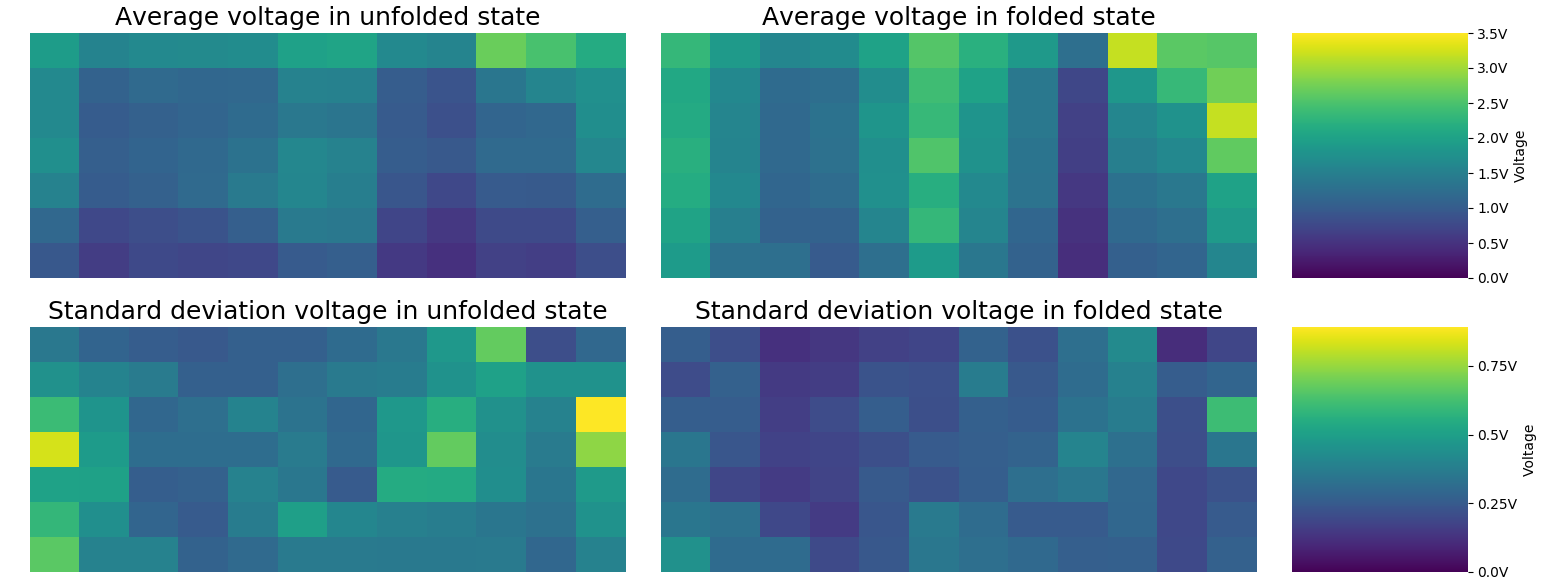
\includegraphics[width=\textwidth, keepaspectratio]{figures/sensor_data_over_states.png}
    \caption{The average and standard deviation of the collected data from the 12 by 7 tactile cells show a higher voltage in the center column---where the fold is---when the cloth is in the folded state. These~figures qualitatively indicate that the tactile cells in the textile react to different folding configurations. }
    \label{fig:sensor_data}
\end{figure}

The classifier was trained using logistic regression with l2-norm regularization on \qty{1418}{} training samples in a five-fold cross-validation setting. The regularization parameter was optimized by performing a random search and by using the F1-score as a performance metric. In order to verify the usability of the classifier, we tested it on an unseen test set of \qty{511} samples which resulted in an average F1-score of \qty{0.97}{}. The full results of the test set are summarized in \cref{table:classifier_results}.

\begin{table}[htpb]
    \centering
    \caption{Test set results of the linear classifier that detects whether the cloth has been folded (511 samples).}
    \label{table:classifier_results}
    \begin{tabular}{@{} ccccc @{}}
        \toprule
                 & Samples & Precision & Recall & F1-score \\
        \midrule
        Unfolded & 342     & 0.98      & 0.98   & 0.98     \\
        Folded   & 169     & 0.96      & 0.95   & 0.96     \\
        \bottomrule
    \end{tabular}
\end{table}

We are able to classify different shape configurations for the textile piece with high accuracy, making the smart textile useful for learning purposes. Other desired features such as wrinkle detection are hard to measure with this technology given the limited sensitivity of the piezoresistive rubber.

%===============================================================================

\section{Results on learning to fold an instrumented cloth}\label{sec:instrumentation_results}

As described in \cref{sec:instrumentation_robotic_setup}, the task consists of folding a rectangular textile piece by using a low-cost dual robotic arm. The arms are positioned in an opposing manner to avoid a collision. In order to avoid damaging the smart textile, we limited the movement of each robot arm to three degrees of freedom~(DOF) instead of the available five~DOF. Consequently, the movements of the robots are limited to one plane.

In order to find the control policy for folding, we formulated the problem as a fitted Q-learning problem \autocite{Watkins1992}. The state-space $S=\mathbb{R}^6$ is defined by the joint space of the dual-arm robot, with six motor angels in total. For each joint, we define two actions: $\pm \Delta$ with $\Delta$ equal to \qty{4}{\degree}. The reward function $R$ is sparse and defined by
\begin{equation} \label{eq:instr_reward_function}
    R=
    \begin{cases}
        100 & \text{on success}            \\
        -1  & \text{penalty for wandering}
    \end{cases}
\end{equation}

We approximate the Q-function with a simple MLP with six input neurons (one for each of the controlled joints), two hidden layers with 128 and 64 ReLu neurons, respectively, and \qty{12}{} output (linear) neurons (one for each of the possible actions). In order to find a good set of parameters, we implemented a simple forward kinematic model of the robot arms in a reaching task setting. This allowed us to sweep across various hyperparameter settings. The optimizer we used is stochastic gradient descent with a learning rate of \qty{0.01}{} and batch size of \qty{64}{} samples. The target network is updated each \qty{1000}{} steps. Exploration is done using an $\epsilon$-softmax policy with \qty{5000}{} exploration steps. Thus, the agent will first execute fully random motor actions and gradually start choosing actions that maximize the expected q-values.

After the selection of the hyperparameters, we trained our dual robotic arm setup from scratch in the real world. As shown in \cref{sub@fig:instrumentation_results_success_rate}, after approximately 60 episodes (\qty{17000}{} steps, or \qty{8}{\hour}), the robot successfully learned to complete the folding task. \cref{sub@fig:instrumentation_results_steps} shows the number of steps the robot needs to fold the cloth per episode. The low dimensional state space of the agent and the learned reward function from tactile information using supervised learning allows the agent to learn to fold the cloth after relatively few training examples.

An example trajectory of the learned policy is shown in \cref{fig:robot_success_merge}. The action probabilities show that at the start of the episode, the agent primarily moves the shoulder joints, as they lead to the largest movement of the end-effector. This behaviour has the benefit that it minimizes the penalty associated with wandering or other suboptimal movements. As the episode progresses, the agent has a higher probability of actuating the elbow and end-effector motors for more refined movement. The~end-effector trajectories, shown in yellow, are not smooth given that the policy is an action probability function calculated over the Q-values of the neural network. Because there are multiple reaching points in the plane to fold the cloth, the agent has multiple options to move during the first part of the episode, leading to jagged end-effector trajectories.

As our experiment illustrates, it is possible to avoid the need for complex vision-based state estimation to learn difficult tasks such as the folding of clothing with low-cost robots. The use of other input modalities such as a smart textile allows a reward function to be learned with simple linear models and is applicable to use for learning on real robotic platforms.

\begin{figure}[htpb]{}
    \centering
    \begin{subfigure}[b][]{0.9\textwidth}
        \centering
        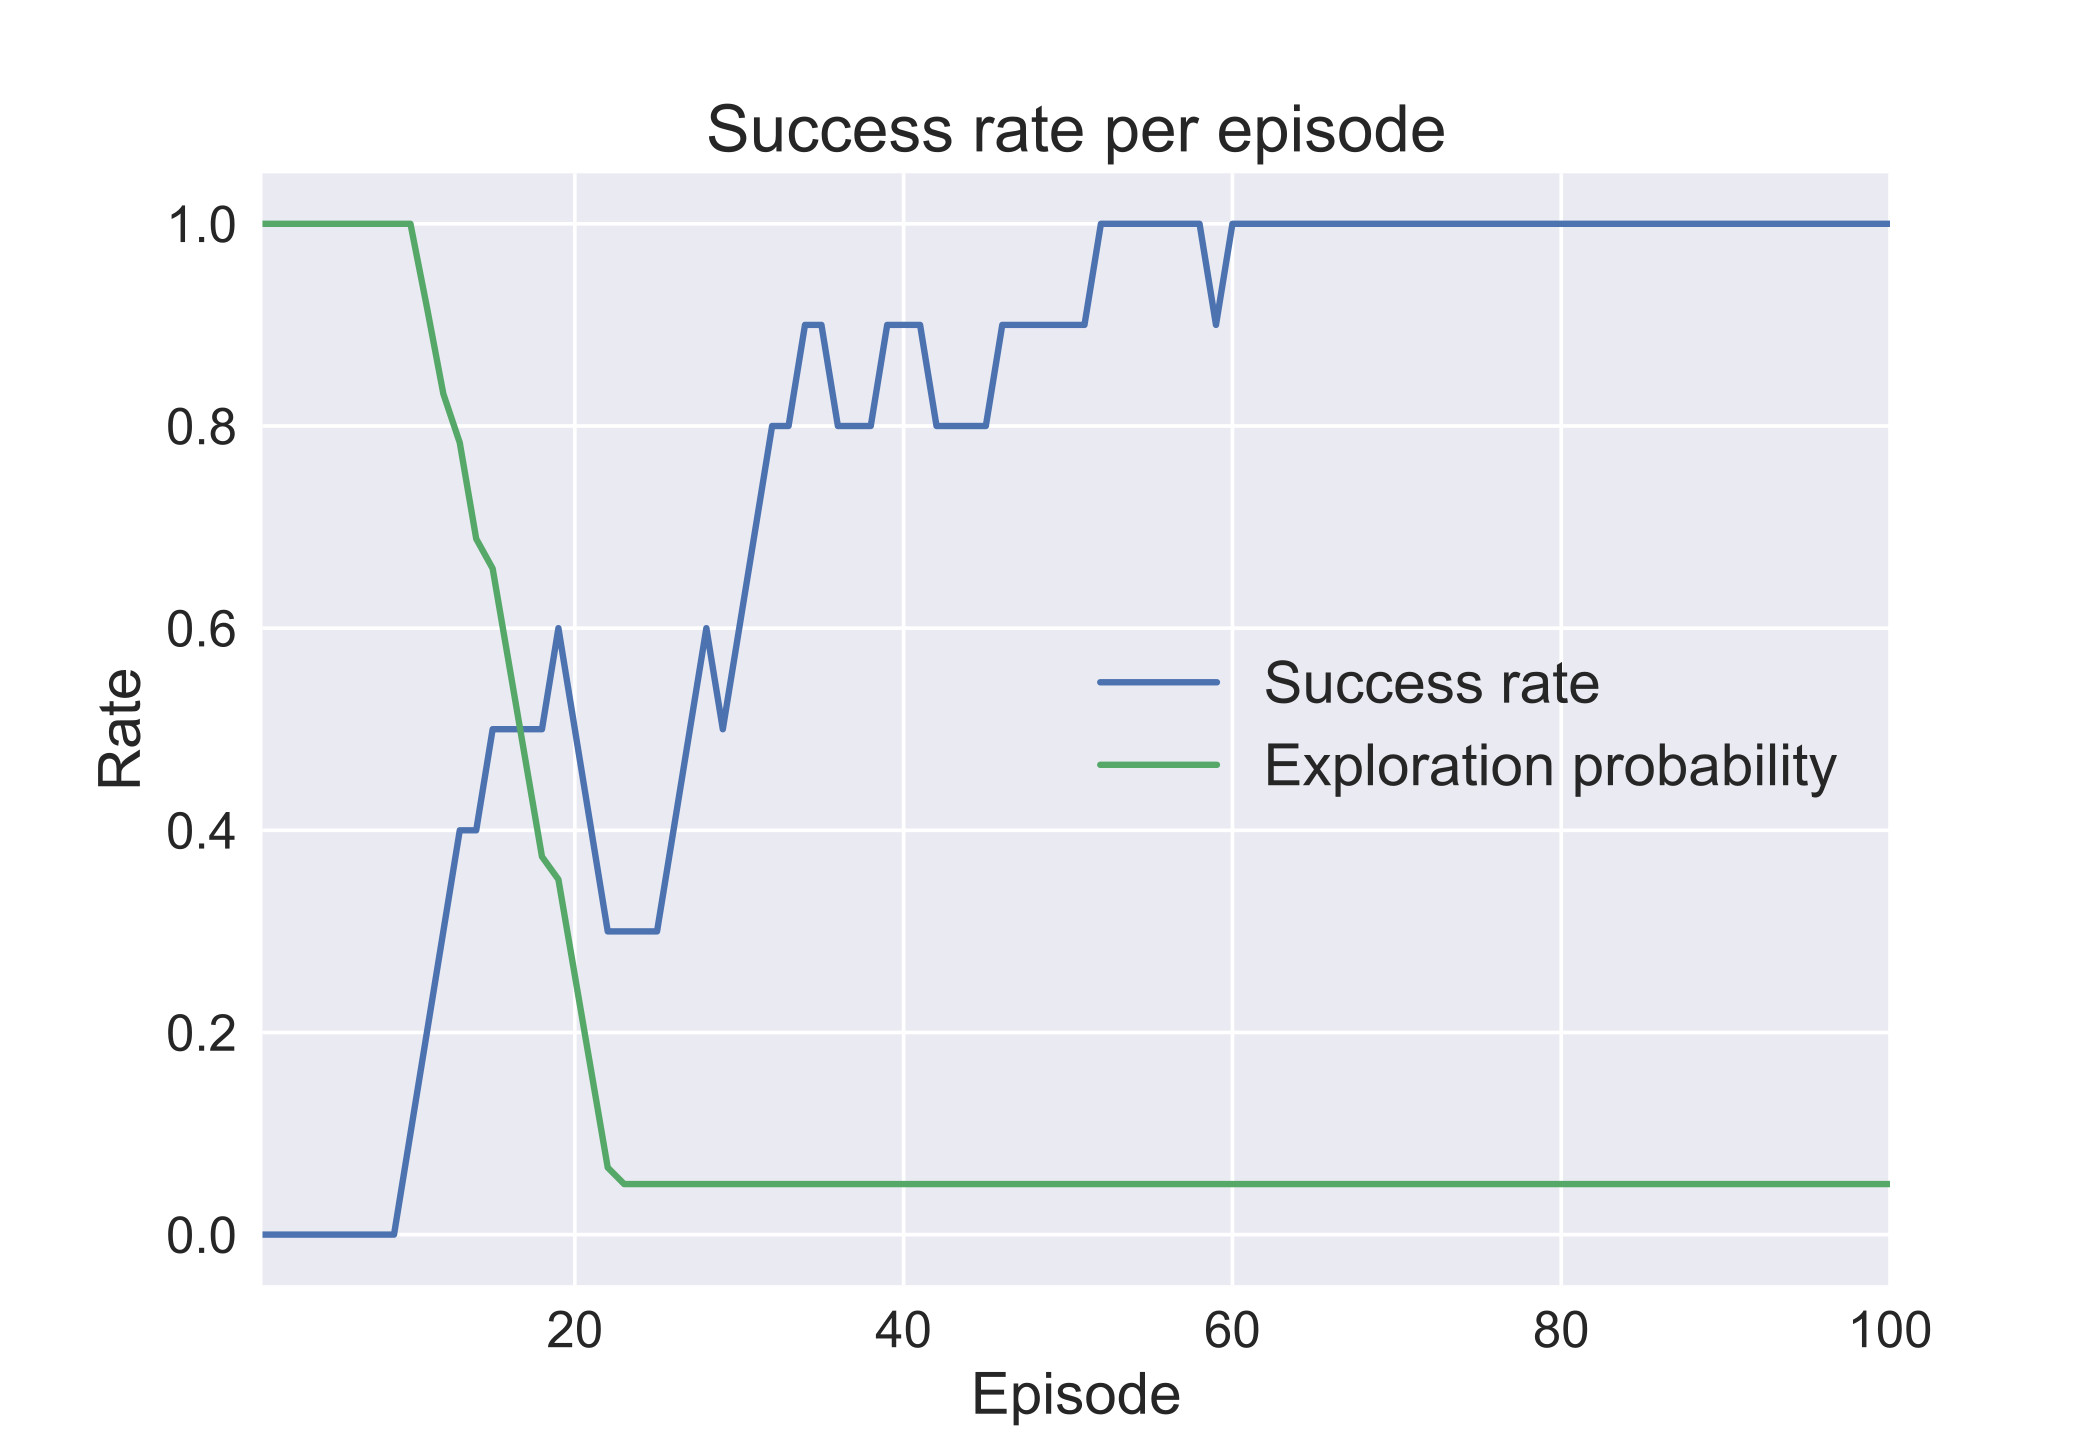
\includegraphics[width=\linewidth]{figures/avg-success-rate.jpg}
        \caption{The folding success rate and exploration probability per episode. The success rate grows to $100\%$ after training for $8$ h on the real robot.}
        \label{fig:instrumentation_results_success_rate}
    \end{subfigure}

    \begin{subfigure}[b][]{0.9\textwidth}
        \centering
        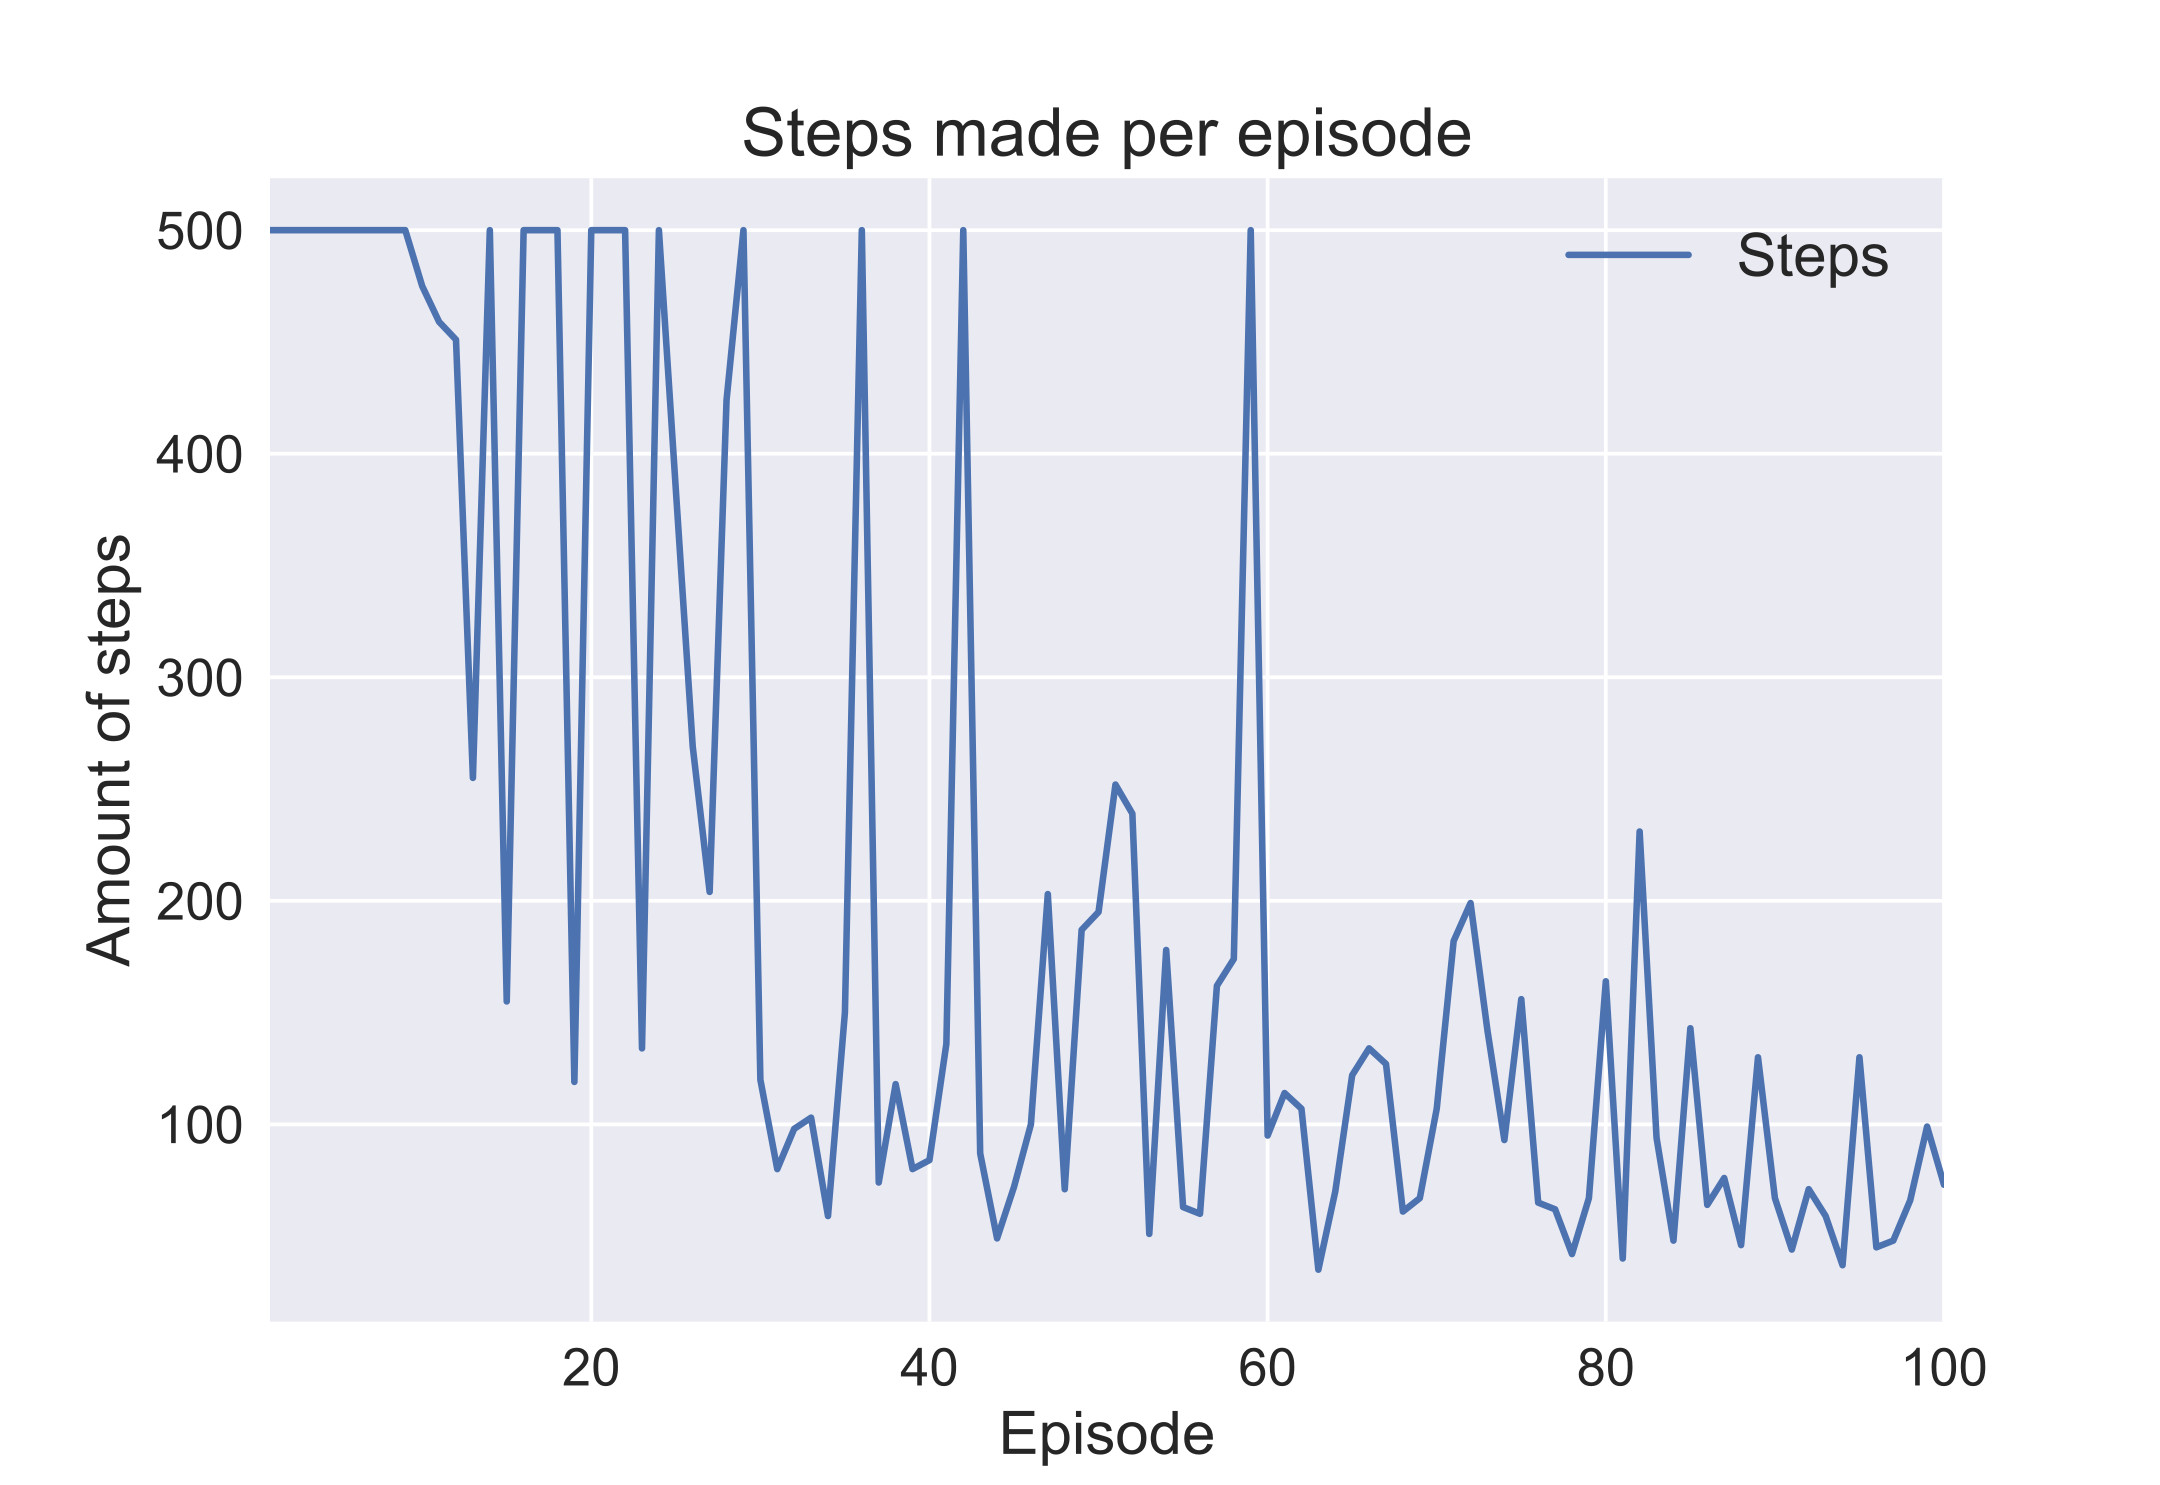
\includegraphics[width=\linewidth]{figures/steps.jpg}
        \caption{The amount of steps required per episode to solve the task; the amount of motor commands needed to fold the cloth decreases after relatively few training examples.}
        \label{fig:instrumentation_results_steps}
    \end{subfigure}

    \caption{Results of training the real robot from scratch to learn how to fold a smart textile.}
    \label{fig:instrumentation_results}
\end{figure}

\begin{figure}[htpb]
    \centering
    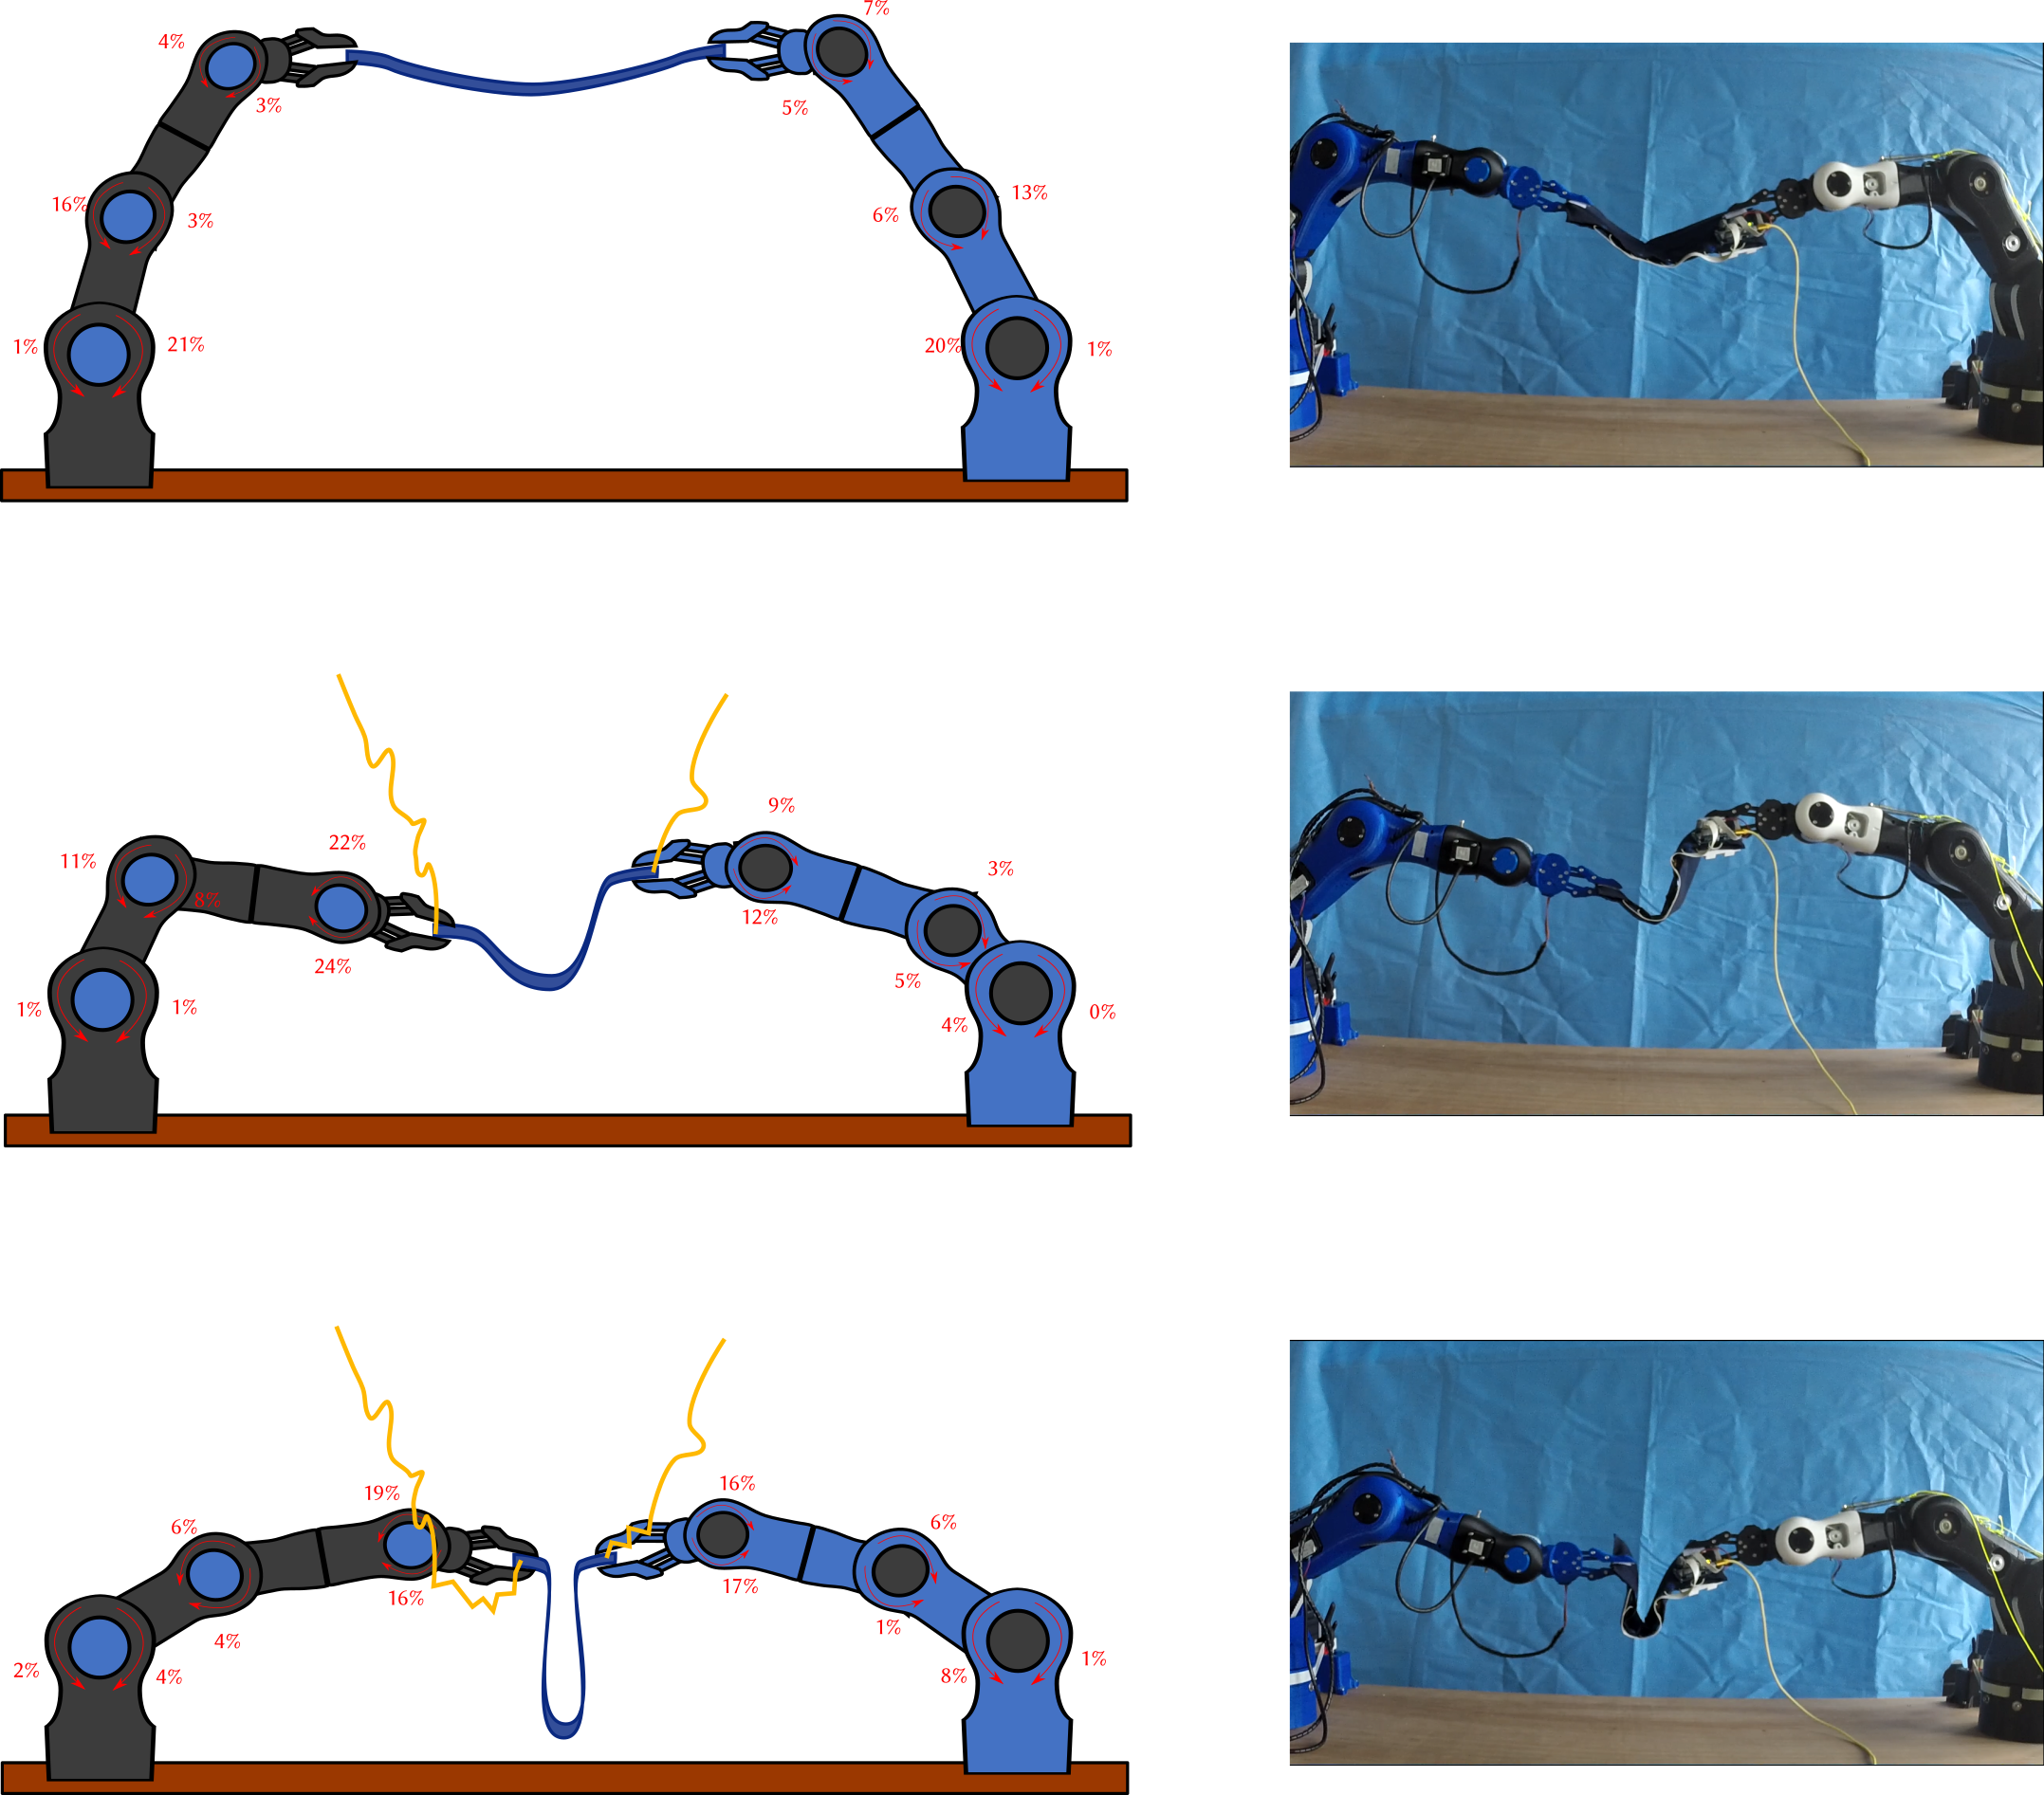
\includegraphics[width=\textwidth, keepaspectratio]{figures/robot_success_merge_with_pics.png}
    \caption{Demonstration of a folding trajectory of the learned policy broken down into three steps: start, middle and end of the episode. The robot state on the figure is visible from the stance of the robot arms. The action probabilities are given in red next to each joint. The executed trajectory is shown with a yellow line.  }
    \label{fig:robot_success_merge}
\end{figure}

%===============================================================================

\section{Discussion} \label{sec:instrumentation_discussion}

\subsection{Grippers for cloth manipulation}
The task we solved in this setup was essentially one of low complexity to demonstrate the applications of accessible sensing technology. When considering more complex cloth-related tasks like grasping and flattening, the question of which gripper design is appropriate arises. We have experimented with different underactuated designs, illustrated in \cref{fig:instr_alternative_grippers}. However, it is non-trivial to determine what types of end effectors and grasps are needed for optimally manipulating cloth-like objects.
Recently, \textcite{Borras2020} provided a holistic overview of the known gripper designs for manipulating textile.
In this work, a systematic classification of grasps in the cloth literature is given based on opposing geometric primitives.
Their work brings the important observation that most prior research uses a pinch grasp with both general-purpose and specialized cloth-specific grippers.
The proposed framework is used to demonstrate that adapting the gripper type to the cloth manipulation task lead to more robust control. We believe this initiative to be a good starting point before resorting to arbitrary cloth manipulation tasks with off-the-shelf parallel grippers.

\newcommand\gripperPicHeight{0.22\textheight}

\begin{figure}[p]
    \centering
    \begin{subfigure}[c]{0.49\textwidth}
        \centering
        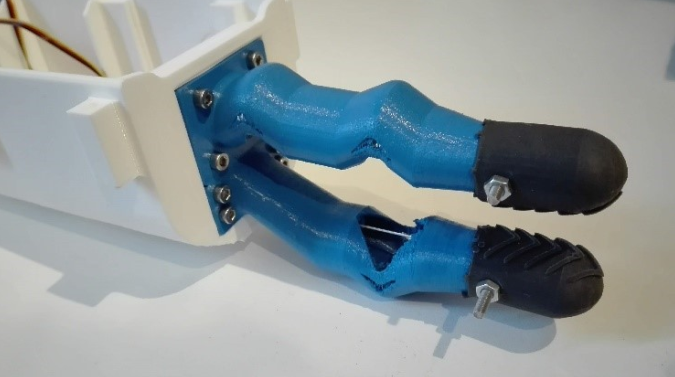
\includegraphics[width=\textwidth,height=\gripperPicHeight]{\home/chapters/06-instrumentation/figures/grippers/gripper-flex}
        \caption{Underactuated finger printed with flexible PLA material.}
        \label{fig:instr_gripper_flex}
    \end{subfigure}
    \hfill
    \begin{subfigure}[c]{0.49\textwidth}
        \centering
        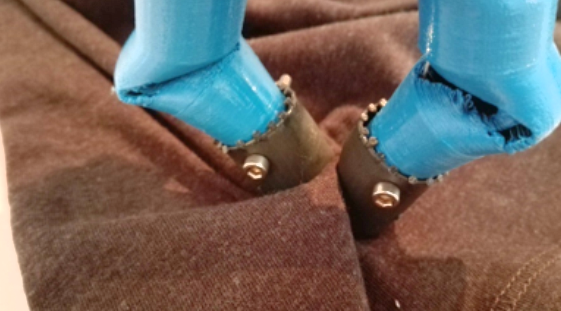
\includegraphics[width=\textwidth,height=\gripperPicHeight]{\home/chapters/06-instrumentation/figures/grippers/gripper-flex-grasp}
        \caption{Finger tips with profile to increase friction for grasping.}
        \label{fig:instr_gripper_flex_grasp}
    \end{subfigure}

    \vskip\baselineskip

    \begin{subfigure}[c]{0.49\textwidth}
        \centering
        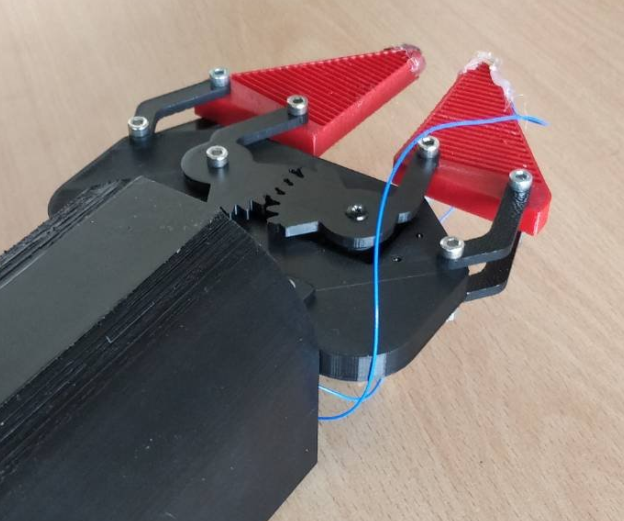
\includegraphics[width=\textwidth,height=\gripperPicHeight]{\home/chapters/06-instrumentation/figures/grippers/gripper-finray}
        \caption{Gripper based on the deformation of the fin of a fish \autocite{crooks2016fin}.}
        \label{fig:instr_gripper_finray}
    \end{subfigure}
    \hfill
    \begin{subfigure}[c]{0.49\textwidth}
        \centering
        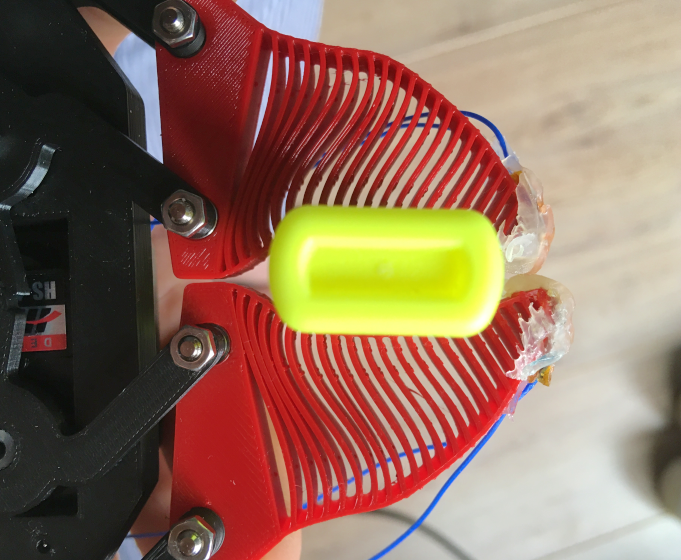
\includegraphics[width=\textwidth,height=\gripperPicHeight]{\home/chapters/06-instrumentation/figures/grippers/gripper-finray-grasp}
        \caption{Compliance increases safety and adapts to the shape of the object.}
        \label{fig:instr_gripper_finray_grasp}
    \end{subfigure}

    \vskip\baselineskip

    \begin{subfigure}[c]{0.49\textwidth}
        \centering
        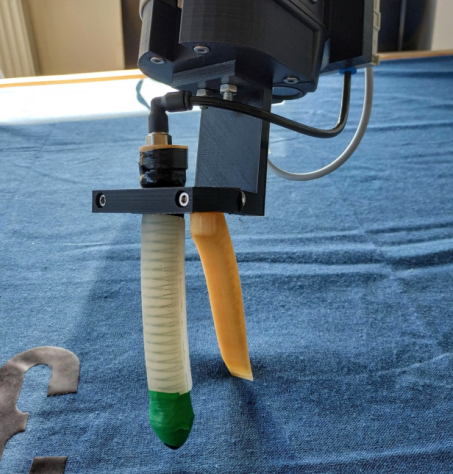
\includegraphics[width=\textwidth,height=\gripperPicHeight]{\home/chapters/06-instrumentation/figures/grippers/gripper-pneu}
        \caption{Pneumatic gripper.}
        \label{fig:instr_gripper_pneu}
    \end{subfigure}
    \hfill
    \begin{subfigure}[c]{0.49\textwidth}
        \centering
        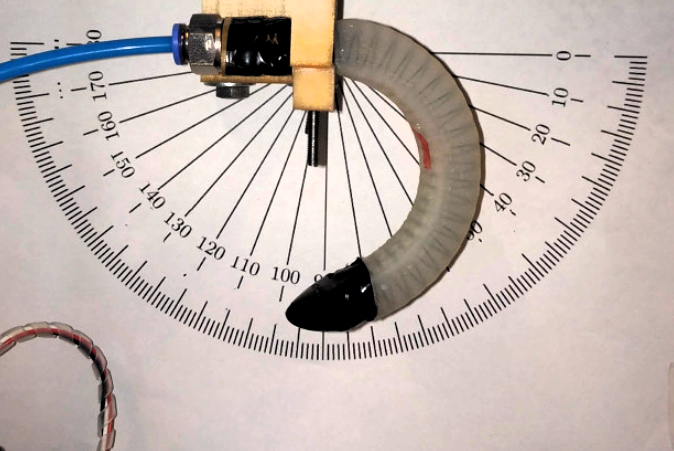
\includegraphics[width=\textwidth,height=\gripperPicHeight]{\home/chapters/06-instrumentation/figures/grippers/gripper-pneu-bend}
        \caption{Bending range.}
        \label{fig:instr_gripper_pneu_bend}
    \end{subfigure}

    \caption[]{Alternative gripper designs we experimented with for cloth manipulation tasks. In collaboration with Peter Verdru, Robbe Nuyttens and Stijn Fierens, former master students at our lab.}
    \label{fig:instr_alternative_grippers}
\end{figure}

\subsection{Future improvements}

The instrumented learning process proposed in this chapter is feasible to scale up to other instances of cloth manipulation tasks given the low computational requirements and the tactile sensitivity of the sensor matrix. The accessible fabrication procedure of the smart textile allows the implementation of this technology for any type of clothing, such as shirts and trousers. The influence on the deformable properties of the cloth can be reduced by miniaturizing the electronics, by using conductive thread instead of copper wires, and by only applying tactile cells in crucial areas. The Arduino we mount on the cloth contains unused functionality and can be replaced by a smaller PCB customized for this task.

Future work includes exploiting the sensitivity of the tactile sensor grid to classify more complex cloth configurations and using more powerful, non-linear classifiers compared to the logistic regression model used in this work. Future research should be directed towards fusing the tactile information with visual data in order to generate a database of self-labelled images of arbitrary cloth configurations. These data can be produced by manipulating the cloth while recording its state with cameras. In order to detect and grasp the cloth and train policies that minimize wrinkles, visual feedback will have to be included. A suitable approach for integrating visual and tactile information is to learn a multimodal latent space, as shown in \autocite{Lee2019}. We discuss our ideas for multimodal learning in \cref{ch:towards_robotic_folding}.

% TODO IF TIME LEFT: toevoegen van francis:
% - 1.5.2 kan je eventueel ook nog iets explicieter zeggen wat we nu aan het doen zijn met de verschillende handen en technologieën (denk aan de Yale en Robotiq hand waarvan we vingers gaan vervangen) + technologieën capacitief & piezoresistief en dan voor de instrumentatie komt daar nog extra piezo-gels en IMU bij (+ de voorgaande).


\section{Conclusion} \label{sec:instrumentation_conclusion}

The difficulty in estimating the state of clothes causes problems for robotic vision pipelines and hinders making reward functions for RL.
In this chapter, we proposed a cost-effective and computationally efficient solution for estimating the state of cloth. We have shown that an inexpensive dual robotic platform can learn to fold a textile piece in the real world with neural fitted Q-learning and without reward engineering. This is done by including tactile sensing in the learning process. We have shown that the high sensitivity of the proposed tactile cells allows the capture of arbitrary cloth configurations. We demonstrated that the tactile data can be used to train a simple logistic regression classifier to detect the cloth state; thus, we create a smart textile piece that is able to accurately detect whether it is folded.

We are aware that we will have to integrate vision for the state estimation to scale up our tasks to real clothing. Consequently, we do not advocate vision-free solutions, but we argue for an interdisciplinary approach in which vision, proprioception and tactile information is combined in order to find the simplest solution of state and reward function estimation.

An important bottleneck of the research presented in this chapter can be found in the reward function in \cref{eq:instr_reward_function}. The scalar value received each step, and on completing the task, are arbitrarily chosen. Our experiments from \cref{ch:simulation} also confronted us that the issue of reward shaping (discussed in \cref{ch:lit}) is also present for cloth folding tasks. We believe that learning the reward function from demonstrations may overcome human bias in reward engineering. However, as discussed in \cref{sec:lit_datasets}, the prerequisite for learning is unavailable; there exists no high-quality dataset of people folding clothing. The lack of a folding dataset is tackled in the next chapter.

\end{document}